\chapter{深度前馈网络}
\label{chap:6}
%%%%%%%%%%%%%%%%%%%%%%%%%%%%%%%%%%%%%%%%%%%%%%%%%%%%%%%%%
%%%%%%%%%%%%%%%%%% author:jim1949@163.com %%%%%%%%%%%%%%%
%%%%%%%%%%%%%%%%%% part:6.0-6.2           %%%%%%%%%%%%%%%
%%%%%%%%%%%%%%%%%%%%%%%%%%%%%%%%%%%%%%%%%%%%%%%%%%%%%%%%%

%需要加4张图,然后把6_0_1,2,3,4换成6_1,2,3,4%
\emph{正则度前馈网络}又被称为\emph{前馈神经网络}或\emph{多层感知机}(MLP), 是一种典型的深度学习模型。
一个前馈神经网络的目标是近似一个函数$f^*$。
例如,对于一个分类器而言,$y=f^*(\bm{x})$将x映射到类别$y$。一个前馈网络定义了一个映射$y=f(\bm{x};\bm{\theta})$, 并且学习了导致产生最好的近似函数的参数$\bm{\theta}$的值。

这些模型被叫做是\emph{前馈},因为信息通过从输入$\bm{x}$产生的方程,到用来定义f的中间计算,最后流向输出$\bm{y}$。这里没有那种模型的输出最后输入给自己的\emph{反馈}联系。当扩展了的反馈神经网络包含了反馈节时,他们被叫做\emph{前馈神经网络}(\emph{recurrent neural networks}),这会在第10章将会提到。

前馈网络对于机器学习的从业者及其重要。他们是形成很多重要商业应用的基础。例如,用于图像中的物体识别的卷积网络就是一种特别的反馈网络。前馈网络是在反复网络的道路上一个概念上的里程碑,它推动了很多自然语言的应用。

前馈神经网络被叫做/emph{网络}的原因是因为一般来说,它们被很多不同的方程组合所代表。这个模型与描述函数如何结合的直接循环图有关。例如,我们有3个函数$f^{(1)}$,$f^{(2)}$, 和$f^{(3)}$在链中相连,以形成$f^{(\bm{x})}=f^{(3)}(f^{(2)}(f^{(1)}(\bm{x})))$。
这些链式结构是最经常使用的神经网络结构。在这个例子里面,$f^{(1)}$被叫做神经网络的\emph{第一层},$f^{(2)}$被叫做\emph{第二层},以此类推。链条的总长给了模型的\emph{深度}。“深度学习”的名字就是从这个术语里面来的。前馈网络的最后一层叫做\emph{输出层}。在神经网络的训练中,我们训练$f^{(\bm{x})}$去匹配$f^*{(\bm{x})}$. 训练数据提供给我们有噪声的,估计的$f^*{(\bm{x})}$的例子,并且在不同的训练点被评估。每个例子$\bm{x}$都伴随一个标签$y\approx f^*(\bm{x})$。这些训练的例子直接给定了在每个点$x$输出层应该怎么做;它必须产生近似于y的值。其它层的表现没有被训练数据直接限定。学习算法必须决定如何水用那些层来得到理想的输出,但是训练数据没有说明每个独立的层应该做什么。相反,学习算法必须决定如何使用这些层来最好实现$f^*$的近似。因为训练数据没有展现每层的理想输出,这些层叫做\emph{隐藏层}(\emph{hidden layers})。

最后,这些网络被称作是\emph{神经}的原因是因为它们是基于神经科学基础的。网络的每个隐藏层一般是引入向量值的。那些隐藏层的维数决定了模型的\emph{宽度}。向量的每个元素可以解释成扮演一个类似于神经节的工作。不把层认为是简单的向量到向量的函数,我们也可以认为层由很多平行工作的\emph{单元}组成的,每个单元代表一个向量到标量的函数。每个单元像一个神经节一样,它从很多别的单元接受输入并且计算他自己的启动值。使用很多向量值代表层的想法来自于神经科学。用来计算这些代表的函数$f^(i)(\bm{x})$的选择,也被神经科学关于生物神经能计算的函数发现所引导。然而,现代的神经网络研究被很多数学和工程规则所指导,并且神经网络的目标也不是完美建模大脑。对于前馈网络的最好的认识是函数近似机器,它被设计成实现统计拟合,偶尔从我们对于大脑知道的部分获得一些灵感,而不是作为大脑函数模型。

一种理解前馈网络的方式,是从线性模型开始然后考虑怎样克服它们的缺陷。线性模型,例如逻辑回归和线性回归,就很有火因为它们可能会拟合地很有效和很可靠,要么在闭环方式要么是用凸优化的方式。线性模型也有一个明显的瑕疵:模型容量被线性函数所显,所以模型不能理解任意两个输入变量之间的交流。

为了将线性模型延伸到代表$\bm{x}$的非线性函数,我们可以应用线性模型不仅仅是$\bm{x}$自身,也可以是转换的输入$\phi(\bm{x})$,这里φ是非线性转换。相似地,我们可以应用5.7.2节描述的核心技巧,以得到基于含蓄应用$\phi(\bm{x})$映射的非线性学习算法。我们可以认为$\phi$作为提供一系列形容x的特征值,或者提供x$\bm{x}$的新代表。
问题是之后如何选择映射$\phi$。
\begin{enumerate}
\item 一种选择是使用一个非常通用的$\phi$,例如无限维的$\bm{\phi}$被隐含地用于基于$RBF$核的\emph{kernel machines}。如果$\phi(\bm{x})$有足够高的纬度,我们可以总是有足够的容量来拟合训练集,但是测试集的正则化经常保持不足。非常普通的特征映射,经常只是基于局部平滑,并且不对足够的先验信息编码解决高级的问题。
\item 还有一个方法是手工调制$\bm{\phi}$。这曾是主要的方法,直到深度学习的出现。这个方法要求对于不同的任务需要从业者人类的数十年的努力,需要参与者擅长不同领域例如语音识别或者机器视觉,并且在不同领域之间转换自如。
\item 深度学习的策略是学习$\phi$。在这种方法中,我们有模型$y=f(\bm{x};\bm{\theta}, \bm{\omega})=\phi(\bm{x}; \bm{\theta})^\top \bm{\omega}$。我们现在有参数$\bm{\theta}$去用来从一个很广义的函数类别里面去学习$\bm{\phi}$,和参数$\bm{\omega}$来从$\phi(\bm{x})$映射到期待的输出。这是一个深度前馈网络的例子,其中$\bm{\phi}$定义了隐含层。这个是唯有的三种方法之一,放弃了训练问题的凸性,但是好处更大。在这种方法中,我们把代表参数化为$\phi(\bm{x};\bm{\theta})$并且用优化算法来寻找$\bm{\theta}$以对应好的代表。如果我们希望,这个方法可以通过变得很通用来获得第一种方法的优势——我们通过使用一个很广泛集来做$\phi(\bm{x};\bm{\theta})$ 。这个方法也可以获得第二种方法的优势。人类从业人员可以将他们的知识编码来通过设计他们预计会表现良好的广泛集来帮助正则化。优势在于人类设计师只需要找出一般的合适函数集,而不用精确地找到正确的函数。
\end{enumerate}

这个通用的通过学习特征来改善模型的规则拓展了这章里面描述的前馈网络。这是个深度学习的复现的主题,适用于这本书里面描述的所有种类的模型。前馈网络是这种去学习决定性从缺乏反馈联系的$x$到$y$的映射的规则的应用。之后说的其它模型将会应用这些规则来学习随机映射,学习有反馈的函数,并且学习在一个向量上的概率分布。

我们从一个简单的前馈网络的例子来开始这章。然后,我们将会阐述每个设计决定来部署前馈网络。首先,训练前馈网络需要做出大量的和线性模型相同重要的设计决定:选择优化,成本函数,和输出形式。我们回顾这些基于梯度的学习的基础,然后进一步学习一些对于前馈网络特别的设计决定。前馈网络介绍了隐藏层的概念,并且这个要求我们去选择可以用来计算隐藏层值的\emph{激活函数}(\emph{activation functions})。我们也必须设计网络结构,包括网络里面有多少层,这些层应该怎么相互连接,以及每层里面有多少单位。学习深度神经网络需要计算复杂函数的梯度。我们提出\emph{反向传播}(\emph{back-propagation})算法和它的可以被用来有效计算梯度的现代正则化。最后,我们以一些历史层面来结尾。

\section{实例:学习XOR}
\label{sec:6.1}

为了让前馈网络的想法更加实际,我们先从一个例子开始,这个例子是用完全函数化的前馈网络来实现一个简单的任务:学习$\bf{XOR}$函数。

$\bf{XOR}$函数(“异或”)是两个二进制数$x_1$和$x_2$的运算。当正好这些二进制其中的一个数等于1,$\bf{XOR}$函数会返回1.否则,它会返回0。$\bf{XOR}$函数提供我们想要学习的目标函数$y=f^*(\bf{x})$。我们的模型提供函数$y=f(bf{x};bf{\theta})$并且我们学习的算法也会修改参数$\theta$,以使f尽可能接近$f^*$。

在这个简单的实例里面,我们不会担心数据正则化。我们想要我们的网络在四个点$\SetX=\{[0,0]^\top,[0,1]^\top,[1,0]^\top,[1,1]^\top\}$上正确地表现。我们将会在这四个点上面训练网络。唯一的挑战是拟合训练集。

我们可以把这个问题处理成回归问题,并且使用一个均方误差损失函数。我们用这个损失函数尽可能地来简化这个数学。我们将会在后面看的有对二进制数据建模的更合适的其它方法。

评估我们的全部训练集,$MSE$损失函数是
\begin{equation}
J(\theta)=\frac{1}{4} \sum_{\bf{x}\in \SetX} (f^*(\bf{x})-f(\bf{x};\bf{\theta}))^2
\end{equation}
现在我们必须选择我们的模型的形式,$f(\bf{x};\bf{\theta})$。假设我们选择一个线性模型,其中$\bf{\theta}$由$\bf{\omega}$和$b$组成。我们的模型定义成
\begin{equation}
J(\bf{x};\bf{\omega},b)=\bf{x}^\top \bf{\omega} + b 
\end{equation}

我们可以在封闭模式下最小化$J(\bf{\theta})$,对$\omega$和b使用正规方程。

在解完正常方程以后,我们获得$\bf{\omega}$=$\bf{0}$和$b=\frac{1}{2}$。每个地方线性模型都简单输出0.5。这个为什么发生呢?图 \ref{fig:6_1}展示了一个线性模型如何不能表示$\bf{XOR}$函数。一种方式去解决这个问题是使用一个模型,这个模型学习一个不同的特征空间,在里面一个线性模型能够体现解决方法。

特别地,我们将会介绍一个非常简单的前馈网络,其中有一个隐藏层包含两个隐藏单元。在图\ref{fig:6_2}中有这个模型的解释。这个前馈网络有一个隐藏单元$\bf{h}$,它是被函数$f^{(1)}(\bf{x};\bf{W},\bf{c})$。这些隐藏单元的值之后被用作第二层的输入。第二层是网络的输出层。输出层仍然只是一个线性回归模型,但是现在他将要应用到h上面而不是x。这个网络现在总共包含两个函数链:$\emph{h}=f^{(1)}(\bf{x};\bf{W},\bf{c})$和$y=f^{(2)}(\bf{h};\bf{\omega},b)$,其中有完整的模型是$f(\bf{x};\bf{W},\bf{c},\bf{\omega},b) = f^{(2)}(f^{(1)}(\bf{x}))$。

$f^{(1)}$应该计算什么样的函数呢?线性模型目前我们已经应用的很好了,并且可能最好也让$f^{(1)}$变成线性的。不幸的是如果$f^{(1)}$是线性的,那么前馈网络作为整体应该保持作为一个输入的线性函数。忽略掉目前的截距项,假设$f^{(1)}(\bf{x})=\bf{W}^\top \bf{x}$,并且$f^{(2)}(\bf{h})=\bf{h}^\top \bf{\omega}$。然后$f(\bf{\omega})=\bf{\omega}^\top \bf{W}^\top \bf{x}$。我们可以代表这个函数为$f(\bf{x})=\bf{x}^\top \bf{\omega’}$ 其中$\bf{\omega’}=\bf{W} \bf{\omega}$。


\begin{figure}[htbp] %  figure placement: here, top, bottom, or page
   \centering
   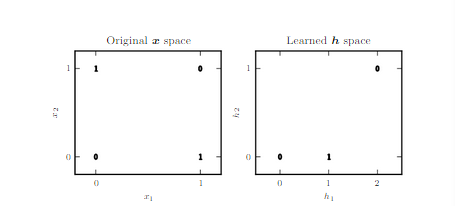
\includegraphics[width=6in]{fig/chap6/6_1.png} 
   \centering
   \caption{学习代表来解决$\bf{XOR}$问题。图像上打印的黑体字指出学习函数在每个点必须输出的值。(\emph{左边})一个线性模型直接应用到最开始的输入不能实现$\bf{XOR}$函数。当$x_1=0$,模型的输出必须随着$x_2$增长而增长。一个线性模型必须有适用于$x_2$一个固定的系数$w_2$。线性模型因此不能使用$x_1$的值来改变$x_2$上的系数,并且不能解决这个问题。(\emph{右边})在变换空间中,从神经网络中提取出由特征代表,一个线性模型现在可以解决这个问题。在我们的解决实例的方法中,必须有输出1的两点已经收缩成特征空间里面一个单独的点。换句话来说,非线性特征已经同时映射$\bf{x}=[0,1]^\top$和$\bf{x}=[0,1]^\top$到一个特征空间里面的一个单独的点,$\bf{h}=[1,0]^\top$。线性模型现在可以描述函数为在$h_1$中增长和在$h_2$中减少。在这个例子中,学习特征空间的动力只是为了使模型容量更大,这样它可以拟合训练集。在更现实的应用中,学习的代表也可以帮助模型正则化。}
   \label{fig:6_1}
\end{figure}


\begin{figure}[htbp] %  figure placement: here, top, bottom, or page
   \centering
   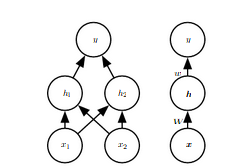
\includegraphics[width=6in]{fig/chap6/6_2.png} 
   \centering
   \caption{使用两种不同方式画出的,一个前馈网络的一个例子。特别地,这是我们用来解决$\bf{XOR}$例子的前馈网络。它有一个包含了两个单元的单隐藏层。(\emph{左边})用这种形式,我们在图中画出每个单元作为一个节点。这个形式是非常明确的和不含糊的,但是对于比这个例子大的网络,就会消耗太多的空间。(\emph{右边})在这个形式中,我们在图中画出一个节点对于每个整个的代表一层的激活部分的矢量。这个形式是更坚实的。有时候我们用描述两层关系的参数名称来注释图中的边缘。这里,我们指出矩阵$\bf{W}$描述着$\bf{x}$到$\bf{h}$的映射,然后向量$\bf{\omega}$描述着$\bf{h}$到$y$的映射。当给这种画图方法贴标签的时候,我们一般删除与各层相关的截距参数。}
   \label{fig:6_2}
\end{figure}

明显地,我们必须使用一个非线性的函数来表示特征。大多数神经网络通过已经学过的参数控制的仿射转换,以及叫作启动函数的一个固定的,非线性的函数做到这样。我们用这里的那个逻辑,定义$\bf{h}=g(\bf{W}^\top \bf{x}+\bf{c})$,这里$\bf{W}$提供了线性变换的权重以及$\bf{c}$作为偏置。之前,为了描述一个线性回归模型,我们用一个权重向量和一个标量偏移参数来描述一个从输入向量到一个输出向量的仿射变换。现在,我们描述一个从向量$\bf{x}$到向量$\bf{h}$的仿射变换,因此我们需要一整个向量的偏置参数。激活函数g一般被选作一个应用来元素加密的函数,有$h_i=g(\bf{x}^\top \bf{W}_{:,i}+c_i)$。在现代神经网络中,默认的推荐是使用在图\ref{fig:6_3}描述的由激活函数$g(z)=\max\{0,z\}$定义的\emph{rectified linear unit}或者ReLU(Jarrett et al., 2009; Nair and Hinton, 2010; Glorot et al., 2011a)。


我们现在可以明确完整的网络为
\begin{equation}
f(\bf{x};\bf{W},bf{c},bf{\omega},\bf{b})=\bf{\omega}^\top \max\{0,\bf{W}^\top \bf{x}+\bf{c}\}+b
\end{equation}

我们可以现在明确对于$\bf{XOR}$问题的解。设
\begin{align}
\bm{W} &= \begin{bmatrix}
1 & 1\\
1 & 1
\end{bmatrix},\\
\bm{c} &= \begin{bmatrix}
0\\
-1
\end{bmatrix},\\
\bm{w} &= \begin{bmatrix}
1\\
-2
\end{bmatrix},
\end{align}
并且b=0。

\begin{figure}[htbp] %  figure placement: here, top, bottom, or page
   \centering
   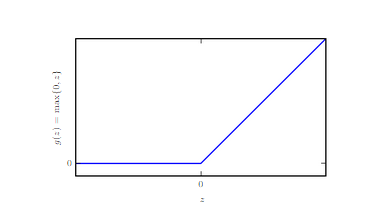
\includegraphics[width=6in]{fig/chap6/6_3.png} 
   \centering
   \caption{修正线性激活函数。这个激活函数是默认的推荐给大多数前馈神经网络使用的激活函数。应用这个函数到线性转换的输出,产生一个非线性转换。然而,这个函数仍然很接近于线性,也就是说他是有两段的分段线性函数。因为修复线性单元几乎是线性的,他们保护了很多的性能使线性模型正则好。一个通用的计算机的原则是我们可以从最小的部分里面构建复杂系统。就像图灵机的记忆一样,只需要能存储0或者1,我们可以从修正线性激活函数中,建造一个通用的函数近似器。}
   \label{fig:6_3}
\end{figure}

我们现在可以考虑让模型处理一批输入。让$\bf{X}$成为包含了二进制输入空间中所有4个点的设计矩阵,每个样例一行:
\begin{equation}
\bf{X}=\begin{bmatrix}
0 & 0\\
0 & 1\\
1 & 0\\
1 & 1
\end{bmatrix}
\end{equation}

在神经网络中第一步是将输入矩阵乘上第一层的权重矩阵:
\begin{equation}
\bf{X} \bf{W}=\begin{bmatrix}
0 & 0\\
1 & 1\\
1 & 1\\
2 & 2
\end{bmatrix}
\end{equation}

下一步,我们加上偏置向量$\bf{c}$,来获得
\begin{equation}
\begin{bmatrix}
0 & -1\\
1 & 0\\
1 & 0\\
2 & 1
\end{bmatrix}
\end{equation}

在这个空间里,所有的样例都在斜率为1的直线上。当我们在这条线上移动的时候,输出需要从0开始, 然后升到1,之后再降到0。一个线性模型不能实现这个函数。为了计算完每个样例的$\bf{h}$的值,我们应用修正线性变换:
\begin{equation}
\begin{bmatrix}
0 & 0\\
1 & 0\\
1 & 0\\
2 & 1
\end{bmatrix}
\end{equation}
这个变换已经改变了样例之间的关系。他们不再在单个线上了。就像图\ref{fig:6_1}所示,它们现在在一个空间中,这里线性模型可以解决问题。

我们通过乘上权重向量$\bf{w}$完成:

\begin{equation}
\begin{bmatrix}
0 \\
1 \\
1 \\
0
\end{bmatrix}
\end{equation}

神经网络已经从这批的每个样例中获得了正确的答案。

在这个样例中,我们简单地简化解,然后显示了它没有错误。在实际情况下,就会有很多的模型参数和很多训练样例,所以人们不能简单像我们这样猜到解。相反,一个基于梯度的优化算法可以找到会制造很少错误的参数。我们对于$\bf{XOR}$描述的解是在损失函数的一个全局最小值,所以梯度下降可以收敛到这个点。也有别的$\bf{XOR}$相同的解,梯度下降也可以找到。梯度下降的收敛点依赖于参数的起始值。在实际中,梯度下降一般不会找到像我们这里展示的一样的干净的,容易理解的整数解。

\section{基于梯度的学习}
\label{sec:6.2}

设计和训练一个神经网络和用梯度下降法训练任何其它的机器学习模型没有太大的区别。在\ref{sec:5.10}节里,我们描述了怎样去通过明确一个优化程序,一个代价函数和一个模型族来构建一个机器学习算法。

我们目前的线性模型和神经网络的最大的区别是神经网络的非线性造成大多数我们感兴趣的损失函数变成了非凸的。这意味着神经网络一般通过迭代的,基于梯度的仅仅驱使损失函数到一个很小的值的优化器来训练,而不是用来训练线性回归模型的线性方程解,或者用来训练逻辑回归或者SVMs的全局收敛保障的凸优化算法。凸优化收敛始于任何起始参数(理论上——实际上它有很强的健壮性但是会遇到数字问题)。随机的梯度下降应用到非凸损失函数没有收敛保障,并且是对于起始参数的值敏感的。对于前馈神经网络来说,初始化小的随机值的所有权重是重要的。偏置也许被起始化为0或者是小的正值。用来训练前馈网络和几乎所有其它的深度网络的迭代的基于梯度的优化算法将会在第八章被详细地描述,其中参数初始化将会被特别地在\ref{sec:8.4}节讨论。目前,不难理解训练算法几乎总是基于用梯度用各种方式来降低代价函数。这个特别的算法是梯度下降方法思想的提升和精炼,在\ref{sec:4.3}节有描述,并且,更具体的,通常是随机梯度下降算法的提高,在\ref{sec:5.9}节有介绍。

我们当然可以训练模型例如线性回归和有梯度下降的支持向量机,事实上当训练集极其大时这是很常见的。从这个观点来看,训练一个神经网络和训练任何其它的模型没有什么太大的区别。计算梯度对于神经网络来说有稍微有点复杂,但是仍然可以被有效和精确地完成。\ref{sec:6.5}节将会描述如何通过方向传播和方向传播算法的现代正则来得到下降。

正如其它机器学习模型一样,为了应用基于梯度的学习我们必须选择一个代价函数,并且我们必须选择如何代表模型的输出。我们现在重新回到这些在神经网络情景有特殊重点的设计考虑上来。

\subsection{代价函数}
\label{sec:6.2.1}

一个深度神经网络设计的重要方面是代价函数的选择。幸运的,神经网络的代价函数或多或少和其它参数模型,例如线性模型的代价函数一样。

在大多数情况,我们的参数模型定义了一个分布$p(\bf{y}|\bf{x};\bf{\theta})$并且我们简单使用最大可能性的原则。这意味着我们在训练数据和如代价函数一样的模型的预计之间使用交互熵。

有时候,我们使用更简单的方法,而不是预测一个完全在$\bf{y}$上的概率分布,我们仅仅预测一些条件为$\bf{x}$的$\bf{y}$的一些统计数字。特殊的代价函数允许我们去训练这些估计的预测值。

用来训练神经网络的整体的代价函数将会经常使这里描述的初始的代价函数和一个规则化因素结合。在第\ref{sec:5.2.2}节,我们已经见到了一些简单的用于线性模型的规则化的例子。用于线性模型的权值衰减方法也是直接适用在深度神经网络,并且是最受欢迎的正则化策略。更加高级的神经网络的正则化策略将在第7章中描述。

\subsubsection{使用最大似然法学习条件分布}
\label{sec:6.2.1.1}

大多数现代神经网络用最大似然来训练。这意味着代价函数是简单的负数对数似然,或者描述成训练数据和模型分布之间的交互熵。这个代价函数表示为

\begin{equation}
J(\bm{\theta})=-\SetE_{\mathbf{x}, \mathbf{y} \sim \hat{p}_\text{data}} \log p_\text{model} (\bm{y} \mid \bm{x})
\end{equation} 
代价函数的特殊形式依据$\log p_\text{model}$的特殊形式在模型之间中改变。上述方程的拓展通常产生不依靠模型参数的一些因子并且可能会被放弃。例如,正如我们在\ref{sec: 5.5.1}节看到的,如果$p_\text{model}(\bm{y}\mid\bm{x}) = \CalN(\bm{y};f(\bm{x};\bm{\theta}), \bm{I})$, 那么我们恢复均方误差代价,
\begin{equation}
J(\theta) = \frac{1}{2} \SetE_{\RVx, \RVy \sim  \hat{p}_\text{data}} || \bm{y} - f(\bm{x}; \bm{\theta}) ||^2 + \text{const},
\end{equation}

至少换算系数是$\frac{1}{2}$并且一个因子不依赖于$\bm{\theta}$。放弃的常数是记忆高斯分布的分歧,在这种情况下我们不选择参数化。之前,我们看到对输出分布的极大似然估计值和线性模型的均协方差最小值的等价性,但是事实上,等价性成立不考虑$f(\bm{x};\bm{\theta})$预测高斯的均值。

从来自最大可能性的代价函数的这种方法的一个优势是,它移去了为每个模型设计代价函数的负担。明确一个模型$p(\bm{y}\mid\bm{x})$自动决定一个代价函数$\log p(\bm{y}\mid\bm{x})$.
一个贯穿神经网络设计的反复出现的主题是代价函数的梯度必须是足够大的河可预测的,来作为一个对于学习算法的好的指导。饱和函数(变得非常平)低估了这个对象因为她们使得梯度变得非常小。在很多情况下它发生因为激活函数曾经产生隐藏单元的输出或者输出层会饱和。负的对数似然帮助我们在很多问题上避免这种问题。很多输出单元包括一个指数函数,当它的变量是绝对值很大的负值时,是会饱和的。在负的对数似然代价代价函数消除了一些输出单元的指数效果。我们仍然将讨论代价函数之间的交互以及在节\ref{sec: 6.2.2}中输出单元的选择。

用于展现最大似然估计值的交互熵代价的不寻常特性是,当它应用到实际中的模型中时,它通常没有最小值。对于离散输出值,大多数模型是用这种方式参数化地以至于它们不能代表概率0或者1,但是可以无限接近。逻辑回归是这个模型的一个例子。对于实值的输出变量,如果模型可以控制输出分布的密度(例如,通过学习高斯输出分布的反差参数)那么它可能会分配特别大密度到正确的训练集输出,导致互熵逼近负无穷。第7章中描述的正则化技巧提供了很多不同方法来修改学习问题,以至于模型不能在这种情况下获得无限制的反馈。

\subsubsection{学习有条件的统计量 }
\label{sec:6.2.1.2}

与学习一个完全的概率分布$p(\bm{y}\mid\bm{x};\bm{theta})$不同,我们经常想要只学习一个基于x的y的条件统计量。

例如,我们也许有一个预测器$f(\bm{x};\bm{\theta})$,我们想用它来预测$y$的平均值。

如果我们用一个足够有效的神经网络,我们可以把神经网络当作是能够代替任何来自一个广泛的函数集的函数$f$,这个类只被特征所限,例如延续性和无界性而不是有一个特别的参数形式。从这点来看,我们可以视代价函数为一个\emph{functional}而不是一个函数。一个\emph{functional}是一个从函数到实数的映射。我们因此可以认为学习作为选择一个函数而不是仅仅选择一些常识。我们可以设计我们的代价\emph{functional}来在一些我们期待的特定的函数得到最小值。例如,我们可以设计代价\emph{funcitonal},使它的最小值在一个函数上,这个函数映射$\bm{x}$到基于$\bm{x}$的$\bm{y}$的预测值。解决一个关于一个函数的优化问题需要一个数学工具叫作\emph{calculus of variations}(变分法),在第\ref{sec:19.4.2}节已经介绍。这不是很必要去为了理解\emph{calculus of variations}而去理解这章的内容。 目前,唯一必要的是理解\emph{calculus of variations}也许会被用来推导出下面的两个结果。
我们第一个用\emph{calculus of variations}推导的结果是解决优化问题
\begin{equation}
f^* = \underset{f}{\argmin}  \ \SetE_{\RVx, \RVy \sim  p_\text{data}} ||\bm{y}-f(\bm{x})||^2
\end{equation}
得到
\begin{equation}
f^*(\bm{x}) = \SetE_{\RVy\sim p_\text{data}(\bm{y}|\bm{x})} [\bm{y}],
\end{equation}
要求是这个函数在我们要优化的类里。换句话说,如果我们可以从产生分布的真实的数据中训练无穷多的样例,最小化平协方差代价函数产生函数,这个函数对于x的每个值预测y的平均值。
不同的代价函数产生不同的统计量。第二个使用\emph{calculus of variations}推导的结果是
\begin{equation}
f^* = \underset{f}{\argmin} \ \SetE_{\RVx, \RVy \sim  p_\text{data}} ||\bm{y} - f(\bm{x})||_1
\end{equation}
产生一个函数预测对于每个$\bm{x}$的$\bm{y}$的值的\emph{中位数},前提是这样一个函数也许会被我们优化过的函数族所描述。这个代价函数一般被称作\emph{mean absolute error}。

不幸的是,当和基于梯度的优化一起使用时,平均协方差误差和平均绝对误差通常导致差的结果。当和哲学代价函数结合的时候,一些饱和输出单元产生非常小的梯度。这是一个原因为什么互熵代价函数比平均协方差误差或者平均绝对误差更受欢迎,甚至当它没有必要去预测一个整个分布$p(\bm{y}\mid\b{x})$的时候也是如此。

\subsection{输出单元}
\label{sec:6.2.2}

代价函数的选择时和输出单元的选择紧密相关的。大多数情况下,我们简单地利用数据分布和模型分布之间的互熵。如何代表输出的选择决定了互熵函数的形式。

任何可能被用来作为输出的神经网络也可以被用做隐藏单元。这里,我们主要用这些单元作为模型的输出,但是原则上它们也可以在内部使用的。在第\ref{sec:6.3}节,我们将重新看一下这些单元,并且提供关于它们作为隐藏单元使用的额外细节。

通过这个部分,我们假设反馈网络提供一系列的隐藏特征,这些特征被$\bm{h}=f(\bm{x};\bm{\theta})$定义。输出层的角色就会是提供一些额外的变换,从特征到完成网络必须展现的任务。
 
\subsubsection{用于高斯输出分布的线性单元}
\label{sec:6.2.2.1}
一种简单的输出单元是一个基于一个没有非线性存在的仿射变换的输出单元。它们通常被称作线性单元。

给定特征$\bm{h}$,线性输出单元的一层产生一个向量$\hat{\bm{y}}=\bm{W}^\top \bm{h} + \bm{b}$。

线性输出层通常被用来产生线性高斯分布的平均值:
\begin{equation}
p(\bm{y}\mid\bm{x}) = \CalN(\bm{y}; \hat{\bm{y}}, \bm{I} ).
\end{equation} 
最大化对数似然此时等价于最小化均方误差。

最大可能框架使学习高斯的反差也很直接,或者使高斯的反差成为输入的一个函数。然而,协方差对于所有输入来说,必须被限制为正定矩阵。用一个线性输出层来满足这样的限制是困难的,所以一般其它输出层被用来对协方差参数化。对协方差建模的方法马上会在第\ref{sec:6.2.2.4}节描述。
因为线性单元没有饱和,它们对于基于梯度的优化算法没有任何困难,并且可能被用在大量的优化算法中。
 
\subsubsection{用于\emph{Bernoulli}输出分布的Sigmoid单元}
\label{sec:6.2.2.2}
很多任务要求预测一个二元变量y的值。具有两个类的分类问题可以归结为这种形式。

最大似然方法是定义一个基于条件$\bm{x}$上$\bm{y}$的\emph{Bernoulli}分布。

一个\emph{Bernoulli}分布只被一个单个参数定义。神经网络需要只预测$P(y=1 \mid \bm{x})$。为了使这个数字成为一个有效的概率,它必须在区间$[0,1]$里面。

满足这个限制要求一些细致的设计工作。假设我们准备用一个线性单元,并且通过阈值来限定来获得有效的概率:
\begin{equation}
P(y=1 \mid \bm{x}) = \max \left \{ 0, \min \{1, \bm{w}^\top \bm{h}+b \} \right \}.
\end{equation}

这确实定义了一个有效的有条件分布,但是我们不能用梯度下降来有效地训练它。任何时候当$\bm{w}^\top \bm{h}+b$在单元区间以外的时候,与它的参数有关的模型的梯度输出会置$\bm{0}$。$\bm{0}$的梯度一般会有问题的,因为学习算法不再有如何提高相应参数的指导。

确实,最好用别的方法来确保无论模型有错误的答案,总有很大的梯度。这个方法是基于使用sigmoid输出单元与最大似然的结合。

一个sigmoid输出单元被定义为
\begin{equation}
\hat{y} = \sigma \left (\bm{w}^\top \bm{h} + b \right ),
\end{equation}
这里$\sigma$是在第\ref{sec:3.10}节描述的逻辑sigmoid函数。
我们可以认为sigmoid输出单元是有两个部分。首先,它使用一个线性层来计算$z=\bm{w}^\top \bm{h}+b$。然后,它使用sigmoid激活函数把$z$转化到概率中。
我们暂时忽略对于$\bm{x}$的依赖性,只讨论如何使用$z$的值来定义一个$y$上的概率分布。Sigmoid可以通过建造一个非规格化概率分布$\tilde{P}(y)$来被驱动,其中概率的和没有到1。我们之后可以用一个合适的常数来分割来得到一个有效的概率分布。如果我们从一个假设非正则化对数概率在$y$和$z$中是线性的,我们可以取幂来获得那个非正则化的概率。我们之后可以正则发现这产生一个由$z$的\emph{sigmoidal}转换控制的\emph{Bernoulli}分布:
\begin{align}
\log \tilde{P}(y) &= yz,\\
\tilde{P}(y) &= \exp(yz),\\
P(y) &= \frac{\exp(yz)}{\sum_{y' = 0}^1 \exp(y' z)},\\
P(y) &= \sigma((2y-1)z).
\end{align}

基于指数的概率分布和正则化在统计模型文献中是很常见的。定义这样一个二元变量上的分布的变量z被称作\emph{logit}。

这种在对数空间中预测概率的方法可以自然地用最大似然方法学习。因为使用最大似然的代价函数是$-\log P(y\mid\bm{x})$, 在代价函数里面的对数部分抵消了$\emph{sigmoid}$的指数部分。如果没有这种效果,$\emph{sigmoid}$的饱和度可以阻止基于梯度的学习做出更好的改进。一个$\emph{Bernoulli}$的最大似然学习的代价函数被$\emph{sigmoid}$参数化后是
\begin{align}
J(\bm{\theta}) &= -\log P(y\mid\bm{x})\\
&= -\log \sigma ((2y-1)z)\\
&= \zeta((1-2y)z).
\end{align}

推导使用了一些来从节\ref{sec:3.10}的性能。通过重新书写softplus函数的损失,我们可以看出只有当$(1 − 2y)z$取绝对值很大的负值时,它才饱和。只在模型已经有正确答案——当$y=1$或者$z$取绝对值很大的正值,或者$y=0$并且$z$取绝对值很大的负值时才发生饱和。当z有错误的符号,softplus函数的参数,$(1-2y)z$,可以简化为$|z|$。当z有错误的符号,随着$|z|$变大,softplus函数渐进趋向于返回它的参数$|z|$。关于z的导数渐进趋向于$\text{sign}(z)$,所以,对于特别不正确的$z$的限制中,softplus函数一点也没有缩小梯度。这个特性很有用,因为它意味着基于梯度的学习可以很快纠正一个错误的$z$。

当我们使用其它代价函数,例如均方差误差,任何时候$\sigma(z)$饱和的时候,损失可以饱和。当$z$变成绝对值很大的负数,sigmoid激活函数饱和到0,当z变成绝对值很大的正值时,饱和到1。无论什么时候这个发生,梯度可以为了对学习有用而变的很小,不论这个模型有正确的答案或者没有。为了这个原因,最大似然几乎总是来训练sigmoid输出单元的优先的方法。

理论上,sigmoid的对数总是确定的和有限的,因为sigmoid返回值在开区间$(0,1)$之间,而不是使用整个的有效概率$[0,1]$的闭区间。在软件应用中,未来避免数字的问题,最好写下负值的对数似然作为一个z的函数,而不是作为一个函数$\hat{y}=\sigma(z)$。如果sigmoid函数下溢到零,之后对$y$取对数会产生负无穷。

\subsubsection{用于Multinoulli输出分布的softmax单元}
\label{sec:6.2.2.3}
任何时候我们想要表示一个有n个可能值的离散变量的概率分布时,我们可能使用softmax函数。这可能被视为一个被用作表示一个用于二位变量的分布的simoid函数的扩展。

Softmax函数大多数情况下,被用于作为分类器的输出,用来代表在n个不同类上的概率分布。softmax函数比较少地,可以被用在模型自身里面,如果我们希望模型在用于一些内部变量中的n个不同选项中选择。
在二元变量中,我们希望产生一个单独的数

\begin{equation}
\hat{y} = P(y=1\mid\bm{x}).
\end{equation}

因为这个数需要处在0和1之间,并且因为我们希望这个数的对数在用于对数似然的基于梯度的优化时表现良好,我们选择去预测一个数$z=\log \hat{P}(y=1\mid\bm{x})$。对其指数化和归一化给我们一个由$sigmoid$函数控制的$Bernoulli$分布。

为了推广到一个有n个值的离散变量的情况,我们现在需要产生一个向量yˆ,其中yˆ = P(y = i | x)。我们要求不仅yˆ的每个元素处在0与1之间,而且整个向量加在一起为1以至于它代表一个有效概率分布。用于bernoulli分布的同样的方法拓展到multinoulli分布。首先,一个线性层预测非标准化对数概率:
\begin{equation}
\bm{z} = \bm{W}^\top \bm{h}+\bm{b},
\end{equation}
其中$z_i=\log \hat{P}(y=i\mid\bm{x})$。softmax函数可以之后通过对z指数化和归一化来获得预期的y。最终,softmax函数的形式是
\begin{equation}
\text{softmax}(\bm{z})_i = \frac{\exp(z_i)}{\sum_j \exp(z_j)}.
\end{equation}

和\emph{logistic sigmoid}一样,在用最大的对数似然来训练\emph{softmax}来输出一个目标值y时,指数函数表现很好。在这个样例中,我们希望最大化$\log P(\RSy =i; \bm{z})=\log \text{softmax}(\bm{z})_i$。定义关于指数的softmax是自然的因为对数似然里的对数可以抵消$softmax$的指数部分:
\begin{equation}
\log \text{softmax}(\bm{z})_i = z_i - \log \sum_j \exp(z_j).
\label{eq:6.30}
\end{equation}
公式\ref{eq:6.30}里的第一个项显示里输入$z_i$总有对于代价函数的一个直接贡献。因为这个项不饱和,我们知道学习可以处理,即使$z_i$对于第二个项的贡献变得很小。当最大化对数似然,第一项鼓励$z_i$升高,而第二项鼓励所有的$z$压低。为了对第二项有一些直接的理解,$\log\sum_j \exp(z_j)$,观察这项可以粗略地被$\max_j z_j$估计。这种近似是对任何明显少于$\max_j z_j$,$z_k$都是不重要的。我们可以从这个近似中得到的解释是负的对数似然代价函数总是强烈惩罚最积极的不正确的预测。如果正确的答案已经对于softmax有最大的输入时,那么-zi项和$\log\sum_j \exp(z_j) \approx \max_j z_j = z_i$项将大致打消。这个例子之后将要对所有的训练代价贡献很小,它将由其它还没有正确分类的样本决定。

到目前为止,我们只讨论了一个单独的例子。综上,非正规化的最大似然将会驱动模型去学习参数,这些参数会驱动softmax来预测在训练集中观察的每个结果的比率:
\begin{equation}
\text{softmax}(\bm{z}(\bm{x}; \bm{\theta}))_i \approx \frac{\sum_{j=1}^m \bm{1}_{y^{(j)}=i, \bm{x}^{(j)} = \bm{x}}  }{ \sum_{j=1}^{m} \bm{1}_{\bm{x}^{(j)} = \bm{x}} }.
\end{equation}
因为最大似然是一个连续的估计器,这就保证了只要模型簇能表示训练分布,它就一定发生。在实际中,有限的模型容量和不完美的优化将意味着模型只能近似得到这些比率。

很多客观的函数而不是对数似然用softmax函数工作地并不好。具体来说,当指数部分变得绝对值很大的负值时,不用对数来抵消softmax的指数部分的客观的函数不能学习,导致梯度消失。特别地,方差是一个用于softmax单元的损失函数的很差的损失函数,并且甚至当模型能做出高度可惜的不正确的预测时,会失败地训练模型来改变它的输出。(Bridle,1990)。为了理解为什么这些其它的损失函数会失败,我们需要测试softmax函数本身。

像sigmoid,softmax激活函数会饱和。当它的输入是绝对值很大的正值或负值,Sigmoid函数有一个会饱和的单个输出。对于softmax的情况,会有很多输出值。当输入值之间的差别变得很极端时,这些输出值会饱和。当softmax饱和时,很多基于softmax的代价函数也饱和,除非它们能颠倒饱和激活函数。

为了说明softmax函数对于它的输入之间的差异作出响应,观察到softmax输出对于所有输入加上相同的标量值时是不变的:
\begin{equation}
\text{softmax}(\bm{z}) = \text{softmax}(\bm{z}+c).
\end{equation}
使用这个性质,我们可以导出一个softmax的数值上稳定的变量:
\begin{equation}
\text{softmax}(\bm{z}) = \text{softmax}(\bm{z}- \max_i z_i).
\end{equation}
变换后的形式使即使当z包含特别大的或者绝对值极其大的负值时,我们可以只用小的数值上的误差来评估softmax。测试数值稳定的变量,我们发现softmax函数由来自变量偏移$\max_i z_i$的数量驱动。

当相应的输入时最大的($z_i = \max_i z_i$)并且$z_i$比其它所有的输入都大很多时,一个输出$\text{softmax}(\bm{z})_i$饱和到1。当$z_i$不是最大输出并且最大值大很多时,$\text{softmax}(\bm{z})_i$也可以饱和到0。这是Sigmoid单元饱和方式的一般化,并且如果损失函数没有被设计去补偿的话,会导致相似的学习困难。

Softmax函数的$\bm{z}$变量可以被用作两种不同方式来产生。最普通的事简单地让神经网络的一个较早的层输出$\bm{z}$的每个元素,正如上述描述一样使用线性层$\bm{z}={W}^\top\bm{h}+\bm{b}$。虽然很直观,这个方法实际上对于分布过度参数化。$n$个输出的常数必须加一起等于1,意味着只有$n-1$参数是必要的;第$n$个值的概率可能通过从1中减去前$n-1$概率项来得到。我们可以因此我们可以强制要求$\bm{z}$的一个元素是固定的。例如,我们可以要求$z_n=0$。确实,这正是sigmoid单元做的。定义$P(y=1\mid\bm{x})=\sigma(z)$和用一个二维的$\bm{z}$和$z_1=0$定义$P(y=1\mid\bm{x})=\text{softmax}(\bm{z})_1$是等价的。无论是softmax的$n-1$个变量还是$n$个变量的方法可以描述同一对概率分布,但是会有不同的学习机制。在实际中,使用过参数化的版本或者受限制的版本直接没有太大的区别,并且去应用过参数化的版本是更容易的。

从神经科学的观点来看,把softmax看成是创造一种参与其中的单元之间的竞争的形式:softmax输出总是加在一起等于1,所以一个单元中值的增长必然和其它值的降低有关。这被认为皮质里的临近神经元之间存在的侧抑制是类似的。在极端情况下(当最大的$a_i$和其它之间的幅度差异是大的时)它变成了一种\emph{winner-take-all}的形式(其中之一的输出几乎为1,而其它几乎为0)。

“Softmax”的名字会有一点让人产生困扰。函数是比max函数更接近于argmax函数。术语“Soft”来源于softmax函数是连续的和可微的。argmax函数,结果表示为一个\emph{one-hot}向量,是不连续,不可微的。Softmax函数因此提供一个argmax的“softened”版本。相应的最大函数的软化版本是$softmax(\bm{z})^\top \bm{z}$。这可能叫softmax函数“$softargmax$”更好,但是目前的名字是一个确立的习惯。

\subsubsection{其它输出形式}
\label{sec:6.2.2.4}
上述描述的线性的,sigmoid,和softmax输出单元是最常见的。神经网络可以拓展到几乎任何我们希望的输出层中。最大似然的原则为如何为几乎任何输出层设计一个好的代价函数提供了指导。

一般而言,如果我们定义了一个条件分布$p(\bm{y}\mid\bm{x}; \bm{\theta})$,最大似然的原则建议我们使用$-\log p(\bm{y}\mid \bm{x};\bm{\theta})$作为我们的代价函数。

一般而言,我们可以把神经网络看作是代表一个函数$f(\bm{x};\bm{\theta})$。这些函数的输出不是值$y$的直接的预测。相反,$f(\bm{x}:\bm{\theta})=\bm{\omega}$为提供了$y$上的分布参数。我们的损失函数之后可以被解释为$-\log p(\RVy; \bm{\omega}(\bm{x}))$。

例如,我们也许希望学习一个基于$\RVx$的$\RVy$的条件高斯方差。在这个简单的情况,方差$\sigma^2$是恒定不变的,这里又一个闭合形式的表达因为最大似然方差的估计器简单地是观察值$\RVy$和它们的预测值直接的方差的经验平均值。一个不需要要求写特殊情况的代码的计算花费更多的方法,是简单地包括方差作为分布$p(\RVy\mid\bm{x})$的其中一个特性,这个分布被$\bm{\omega}=f(\bm{x};\bm{\theta})$所控制。负对数似然$-\log p(\bm{y};\bm{\omega}(\bm{x}))$之后将提供一个有一个特殊项的损失函数来使我们的最优化过程渐进地学习方差。在标准差不依赖于输入的简单轻快中我们可以在网络中产生一个简单的产生一个新的参数,这个参数直接被复制到$\bm{\omega}$中。这个简单的参数也许是$\sigma$本身,或者可以是代表$\sigma^2$的参数$v$,或者它可以是一个代表$\frac{1}{\sigma^2}$的参数$\beta$,取决于我们如何选择对分布参数化。我们也许希望我们的模型去预测对于$\RVx$的不同的值$\RVy$之中的一个不同数量的方差。这个被叫做heteroscedastic模型。在heteroscedastic情况中,我们简单地让方差的具体值成为$f(\RVx;\bm{theta})$输出的其中一个值。一个典型的方式去做这个是用精度,而不是方差,正如公式\ref{sec:3.2.2}描述的那样,来构建高斯分布。在多维变量的情况中,使用哦一个对角精确矩阵是最常见的。
\begin{equation}
\text{diag}(\bm{\beta}).
\end{equation}
这个公式适用于梯度下降,因为由$\bm{\beta}$参数化的高斯分布的对数似然的公式只涉及$\beta_i$的乘法和$\log \beta_i$的加法。乘法,加法和对数运算的梯度都很好的表现。通过对比,如果我们把输出以方差形式参数化,我们将需要使用除法。除法函数在零附近变得任意陡峭。尽管大的梯度可以帮助学习,任意大的梯度通常导致不稳定。如果我们用标准差把输出参数化,对数似然仍然将会涉及除法,并且也会涉及平方。通过方差运算的梯度会在零附近消失,使学习平方的参数变得困难。
不管我们是否使用标准差,方差,或者精度,我们必须确认高斯的协方差矩阵是正定的。因为精度矩阵的特征值是协方差矩阵的特征值的倒数,这和确定精度矩阵是正定的是等价的。如果我们使用一个对角矩阵,或者一个标量乘以对角矩阵,那么我们唯一需要的条件是去强制使模型的输出都为正。如果我们假设a是被用来决定对角精度的模型的原始激活,我们可以用softplus函数来获得一个正的精度向量:$\bm{\beta}=\zeta(\bm{a})$。如果用方差或者标准差而不是精度或者如果使用一个标量乘以单位矩阵而不是对角矩阵,相同的策略同样适用。

学习一个协方差或者比对角矩阵有更丰富结构的精度矩阵是很少见的。如果协方差矩阵是满的和有条件的,那么参数化的选择保证预测方差矩阵的正定。这可以通过写成$\bm{\Sigma}(\bm{x})=\bm{B}(\bm{x})\bm{B}^\top (\bm{x})$来实现,这里$\bm{B}$是一个无约束的方阵。如果矩阵是满秩的,这个实际问题是计算可能性的代价是昂贵的,一个$d\times d$的矩阵的行列式或者$\bm{\Sigma}(\bm{x})$的逆(或者等价地,更常用地,对它的特征值的分解或者$\bm{B}(x)$的特征值的分解),要求$O(d^3)$的计算量。

我们通常想要实现\emph{multimodal regression},也就是,去预测来源于条件分布$p(\bm{y}\mid\bm{x})$的实值,这个分布对于相同的$\bm{x}$值在$\bm{y}$空间中有不同的峰值。在这种情况下,一个高斯混合是输出的自然表示(Jacobs et al., 1991; Bishop, 1994)。用高斯混合作为它们的输出的神经网络通常被叫做\emph{mixture density networks}(\emph{混合密度网络})。具有$n$的部分的高斯混合输出被条件概率分布定义为
\begin{equation}
p(\bm{y}\mid\bm{x}) = \sum_{i=1}^n p(\RSc = i \mid \bm{x}) \CalN(\bm{y}; \bm{\mu}^{(i)}(\bm{x}), \bm{\Sigma}^{(i)}(\bm{x})).
\end{equation}
神经网络必须有三个输出:一个定义$p(c=i\mid\bm{x})$的向量,一个给所有的$i$提供$\bm{\mu}^{(i)}(\bm{x})$的矩阵,和一个给所有i提供$\bm{\Sigma}^{(i)}(\bm{x})$的张量。这些输出必须满足不同的限制:
\begin{enumerate}
\item 混合部分$p(\RSc=i\mid\bm{x})$:这些形成一个关于隐变量\footnote{我们认为c是隐变量是因为我们没有在数据中观察到它:已知输入$\bm{x}$和目标$\bm{y}$,确切地知道哪个高斯部分产生了$\bm{y}$是不可能的,但是我们可以想象$\bm{y}$是通过挑选其中之一来产生的,并且使那个没有观察到的选择作为随机变量。
}$c$的n个不同部分的\emph{multinoulli distribution},并且通常可以通过一个n维的向量上的softmax来获得,来保证这些输出是正并且和为1。

\item 均值$\mu^(i)(\bm{x})$:这些指明了与第i个高斯部分相连的中心或者均值,并且是无限制的(一般对于这些输出单元根本没有非线性)。如果$\bm{y}$是一个d维向量,那么网络必须输出一个$n\times d$的矩阵,这个矩阵包涵这些n个这种d维向量。用最大似然学习这些均值比只用一个输出模式学习分布的均值复杂一点。我们只想去更新用于实际上产生观测值的部分的均值。在实际情况中,我们不知道每个观测值是哪个部分产生的。负对数似然的表达式自然地对每个样例对于每个部分的概率损失产生的贡献赋予权重,权重值大小由组成部分产生的案例的概率来决定。

\item 协方差$\bm{\Sigma}^{(i)}(\bm{x})$:这些明确了用于每个部分i的方差矩阵。当学习一个单个的高斯部分的时候,我们一般用一个对角矩阵来避免计算行列式。当学习混合的均值,最大似然是复杂的,它需要将每个点的部分责任分配到每个混合部分中。给定了在混合模型下,正确的负对数似然,梯度下降将会自动按照正确的过程。
\end{enumerate}

有报道说有条件高斯混合的基于梯度的诱惑可能是不可靠的,部分是因为设计除法,(除以方差)这可能会数据上的不稳定(当一些方差对于一个特殊的样例变得小的时候,产生很大的梯度)。一个解决方案是clip gradients(在第10.11.1节可以看到),另外一种是梯度启发式收缩。(Murray and Larochelle, 2014)。

高斯混合输出是语音生成模型(Schuster, 1999)中,或者物理物体运动(Graves, 2013)。混合密度策略为网络提供了方式去代表很多输出模型,并且去控制它的输出的方差,这对于获得一个在这些实值区间里的高质量的结果极其重要。一个混合密度网络的样例在图\ref{fig:6_4}中显示。

一般来说,我们可能希望继续去为包含更多变量的更大的向量$\bm{y}$建模,并且去在这些输出变量上施加更多更丰富的结构。例如,我们可能希望对于我们的神经网络,输出组成句子的字符序列。在这些情况中,我们可能继续使用最大似然的原则应用到我们的模型$p(\bm{y};\bm{\omega(\bm{x})})$,但是我们形容$\bm{y}$模型变得太复杂,超过了本章的范围。第10章描述里如何使用循环神经网络来定义序列上的这些模型,并且第III部分描述里对于任意概率分布的建模的高级技巧。

\begin{figure}[htbp] %  figure placement: here, top, bottom, or page
   \centering
   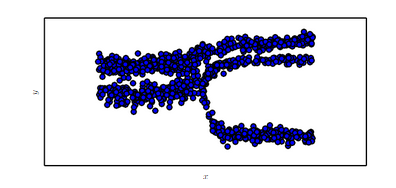
\includegraphics[width=6in]{fig/chap6/6_4.png} 
   \centering
   \caption{样例是用有一个混合密度输出层的神经网络画得。输入x从一个均匀分布中采样,输出y从$p_{\text{model}}(y \mid x)$中采样。神经网络能够学习从输入到输出分布的参数的非线性映射。这些参数涉及了概率,这个概率决定了三个混合部分中的哪个将产生输出和每个混合部分的参数。每个混合部分是有预测的均值和方差的高斯分布。输出分布的所有这些部分能依据输入$x$而变化,并且也在非线性方式中这样做。}
   \label{fig:6_4}
\end{figure}






